\section{Test P4}
En esta sección vamos a seguir el tutorial y los test que proponen la organización de p4 en su repositorio oficial.
\begin{itemize}
    \item \url{https://github.com/p4lang/tutorials}
\end{itemize}
La metodología de los tutoriales consiste en completar el esqueleto del código p4 dado por ellos para hacer funcionar las distintas pruebas. El escenario que se ha empleado para establecer un eviroment de pruebas es Mininet.

\section{Test 1: Implementando el fordwarding básico}

El objetivo de este test es escribir un programa P4 que implemente el fordwarding básico. Con el reenvío de IPv4, el conmutador debe realizar las siguientes acciones para cada paquete:
\begin{itemize}
    \item Actualizar las direcciones MAC de origen y destino.
    \item Disminuir el campo de la cabecera IP (TTL).
    \item Reenviar el empaquete el puerto apropiado.
\end{itemize}

Nuestro switch tendrá una sola tabla, que el plano de control llenará con reglas estáticas. Cada regla asignará una dirección IP a la dirección MAC y al puerto de salida para el próximo salto. Ya se han definido las reglas del plano de control, por lo que solo necesitamos implementar la lógica del plano de datos de nuestro programa P4 (\textit{basic.p4}).

\subsection{Comprobar el modelo suministrado}
En este punto siguiendo el tutorial, tenemos que comprobar como efectivamente el modelo suministrado no es capaz de establecer comunicaciones entre nodos finales. Esto se debe a que el plano de datos de los switches está incompleto, y será nuestra misión la de completar el plano de datos con nuestro programa en p4 que dotará de la capacidad de fordwarding de paquetes a los switches. \newline
\newline
Procedimiento a seguir para llevar a cabo el test:
\begin{itemize}
    \item Hacemos uso del Makefile que trae el tutorial: \textbf{make run}, este target del Makefile automatizará las siguientes tareas:
    \begin{itemize}
        \item Compilará el archivo \textit{basic.p4} para el behavioral model 2 (bm2) el target simple switch
        \item Lanzará Mininet con una topología de tres switch conectados triangularmente y a cada switch se conectará un host. Los host tendrán respectivamente las IPs 10.0.1.1, 10.0.2.2, 10.0.3.3. 
    \end{itemize}
    \item En el mismo directorio se encuentran dos herramientas esritas en Python, servidor y cliente, que nos ayudaran a generar tráfico desde un host a otro. Estas herramientas hacen uso de Scapy para poder visualizar el contenido el paquete generado. Herramientas \textit{receive.py} y \textit{send.py}. 
    \item Levantaremos dos terminales por ejemplo, host 1 y host 2: \textbf{xterm h1 h2}
    \item Ejecutaremos las herramientas para generar tráfico entre ambos host.
    \item El mensaje no llegará, salimos de Mininet con \textbf{exit}, y limpiamos el escenario y Mininet con \textbf{make stop} (Este target llamará a \textbf{sudo mn -c} por nosotros).
\end{itemize}

%%%%%%%%%%%%%%%%%%%%%%%% foto terminales %%%%%%%%%%%%%%%%%%%%%%%%%

\begin{figure}[!htb]
  \centering
    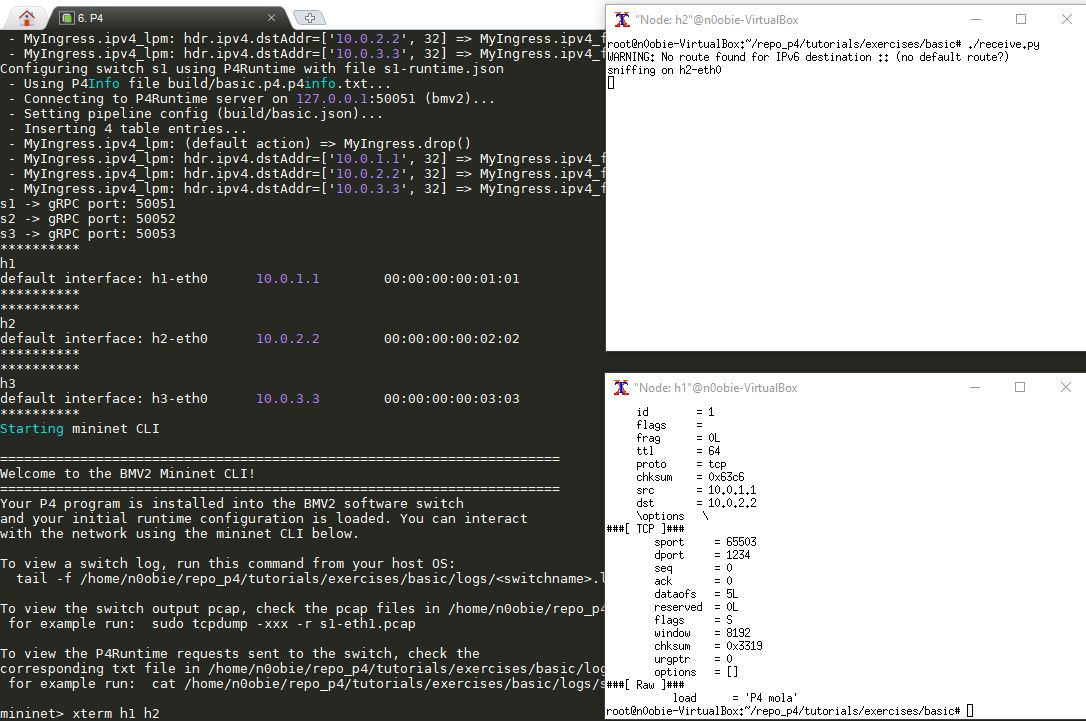
\includegraphics[width=\linewidth]{./img/test/1.JPG}
    \caption{Test Mininet: No llega el mensaje.}
  \label{fig:yo}
\end{figure}

%%%%%%%%%%%%%%%%%%%%%%%% foto terminales %%%%%%%%%%%%%%%%%%%%%%%%%

Un programa P4 define una pipe-line de procesamiento de paquetes, pero las reglas dentro de cada tabla se insertan desde el plano de control. Cuando una regla coincide con un paquete (Hay un hit), su acción se invoca con los parámetros proporcionados por el plano de control como parte de la regla.\newline
\newline
En este test, ya se ha implementado la lógica del plano de control, está suministrado por el equipo de p4. A la hora de levantar la instancia de Mininet, el comando make run instalará las reglas de procesamiento de paquetes en las tablas de cada switch. Estas se definen en los archivos sX-runtime.json, donde X corresponde al número de switch.\newline
\newline
Se hace uso de P4Runtime para instalar las reglas del plano de control. El contenido de los archivos sX-runtime.json se refiere a nombres específicos de tablas, claves y acciones, tal como se define en el archivo P4Info producido por el compilador (busque el archivo build / basic.p4info después de ejecutar make run). Cualquier cambio en el programa P4 que agregue o cambie el nombre de tablas, claves o acciones deberá reflejarse en estos archivos sX-runtime.json.

\subsection{Desarrollo del fordwarding L3}
El archivo basic.p4 contiene un programa P4 esqueleto con piezas lógicas clave donde deberemos completar su cuerpo para el correcto funcionamiento del switch. Las partes que debemos completar son las siguientes:
\begin{itemize}
    \item Completar el Parser para extraer las cabeceras de ethernet e ipv4.
    \item Completar un action llamado forward\_ipv4 que deberá: 
        \begin{itemize}
            \item Establecer el puerto de salida del paquete. 
            \item Establecer como dirección MAC origen la MAC destino de la trama recibida. 
            \item Establecer como dirección MAC destino del paquete la MAC del siguiente salto.
            \item Decrementar el campo TTL de la cabecera ipv4.
        \end{itemize}
    
    \item Completar el campo apply para decidir si aplicar la tabla.
\end{itemize}
\newpage
Para completar el parser de entrada del switch hemos definido tres estados, el primer estado, entry-point, llamado start. El segundo parse\_ethernet, para extraer la cabecera de Ethernet, y decidir si si entramos a la ultima fase del parser, parse\_ipv4, en función del campo etherType. La ultima fase del parser únicamente extrae la cabecera de Ipv4. 
\begin{figure}[!htb]
  \centering
    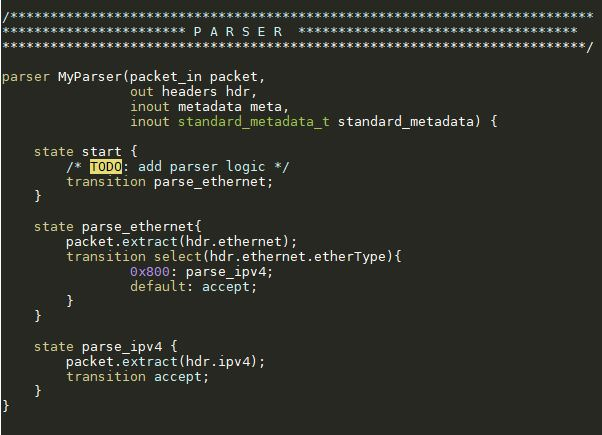
\includegraphics[width=0.8\linewidth]{./img/test/2.JPG}
    \caption{Parser.}
  \label{fig:yo}
\end{figure}
\newline
Hemos definido un action que hacer forwarding a los paquetes que les llega a los switch, deberá especificar un puerto de salida, modificar las MAC para el siguiente hop, y decrementar en uno el campo TTL de la cabecera Ipv4. \newline

\begin{figure}[!htb]
  \centering
    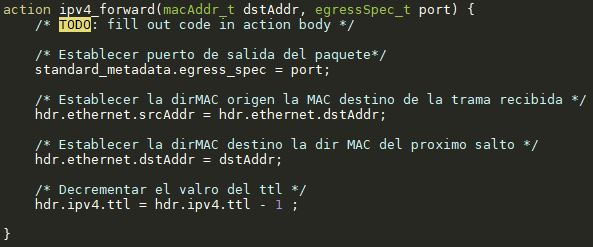
\includegraphics[width=0.8\linewidth]{./img/test/3.JPG}
    \caption{Action forwarding.}
  \label{fig:yo}
\end{figure}
\newline
Según los requerimientos dados, debemos comprobar con anterioridad si existe y es valida la cabecera Ipv4.
\newpage
\begin{figure}[!htb]
  \centering
    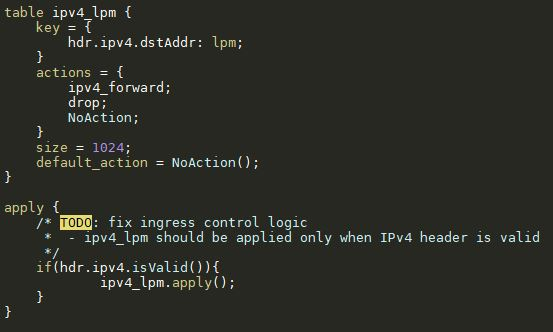
\includegraphics[width=0.7\linewidth]{./img/test/4.JPG}
    \caption{Tabla match-action de nuestro switch.}
  \label{fig:yo}
\end{figure}
Por último, únicamente debemos especificar en el deparser como queremos serializar las cabeceras, y en que orden. A continuación, se incluirá la carga útil y se conformará el paquete. Por carga útil entendemos toda información no procesada por el parser de entrada por el switch p4.
\begin{figure}[!htb]
  \centering
    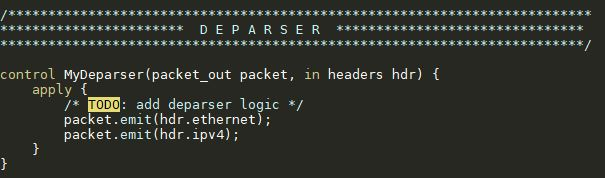
\includegraphics[width=0.8\linewidth]{./img/test/5.JPG}
    \caption{Deparser de nuestro switch.}
  \label{fig:yo}
\end{figure}
\newline
\newline
A continuación, se puede apreciar en la arquitectura conformada en bloques de nuestro switch. Donde, cada bloque va especificando la funcionalidad para la que ha sido programada. Este diseño es muy útil para ver de manera la operativa funcional de nuestro switch.
\newline
\newline
\begin{figure}[!htb]
  \centering
    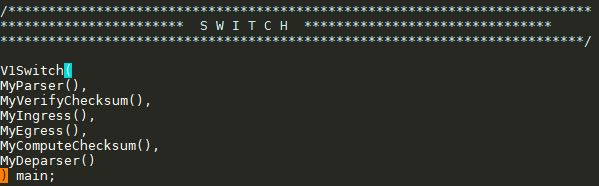
\includegraphics[width=0.8\linewidth]{./img/test/6.JPG}
    \caption{Topología funcional de nuestro switch.}
  \label{fig:yo}
\end{figure}
\newpage
A continuación, se expone como tras implementar los cambios existe conectividad en la topología entre todos los host. Para implementar los cambios antes hemos realizado un \textbf{sudo make stop} y un \textbf{sudo make clean} para limpiar los archivos residuales de los switch p4 y de Mininet.
\begin{figure}[!htb]
  \centering
    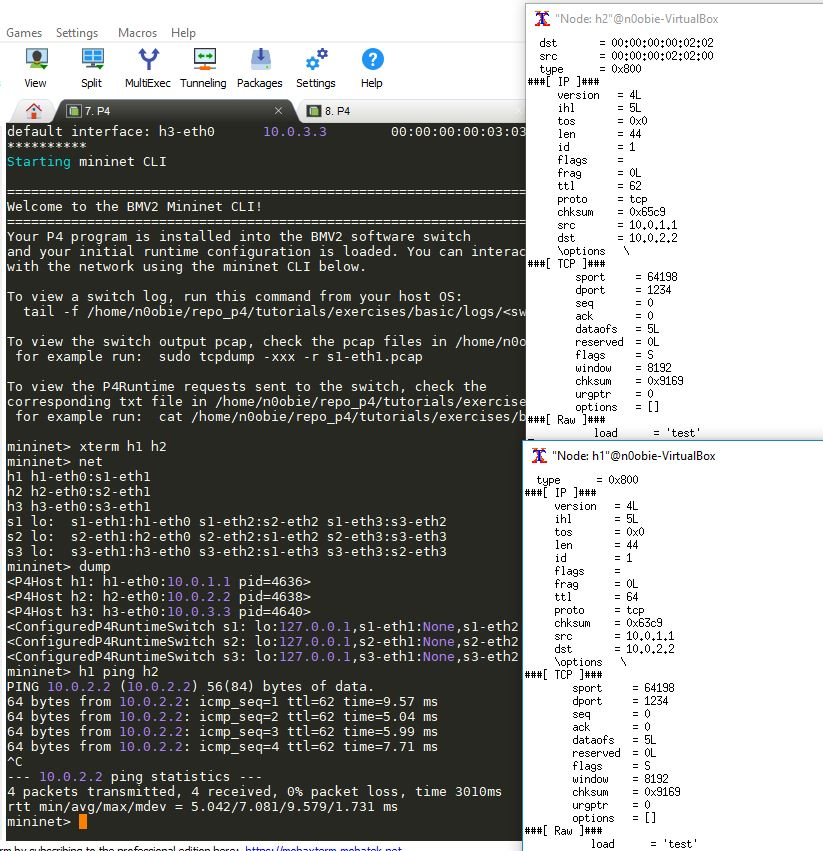
\includegraphics[width=\linewidth]{./img/test/7.JPG}
    \caption{Funcionamiento de switch programado.}
  \label{fig:yo}
\end{figure}
\newpage
\section{Test 2: Implementando el tunelado básico}